\documentclass[xcolor=table]{beamer}
\usepackage[utf8]{inputenc}
\usepackage[T1]{fontenc}
\usepackage[alf]{abntex2cite}	
\usepackage{udesc}
\usepackage{amsfonts,amsmath,amssymb,mathtools}
\usepackage{verbatim}
\usepackage{listings}
\usepackage[ddmmyyyy]{datetime}
\usepackage{hyperref, url}
\usepackage{graphicx}
\usepackage{multirow}
\usepackage{changepage}
\usepackage{pgfplots}
\usepackage{textcomp}
\usepackage{geometry}

\pgfplotsset{width=\textwidth+1.5cm,height=8cm,compat=1.9}

\setbeamertemplate{frametitle continuation}{}

% suprimindo warnings do hyperref
\pdfstringdefDisableCommands{%
  \def\\{}%
  \def\texttt#1{<#1>}%
  \def\smallskip{}%
  \def\medskip{}%
}

\lstset{language=C++,
    basicstyle=\ttfamily,
    keywordstyle=\color{blue}\ttfamily,
    stringstyle=\color{red}\ttfamily,
    commentstyle=\color{gray}\ttfamily,
    morecomment=[l][\color{magenta}]{\#}
}

\renewcommand{\figurename}{Figura}
\renewcommand{\tablename}{Tabela}

\sloppy
\title[]{Trabalho Final de Programação Paralela - Paralelizando Quebra de Chaves do Algoritmo RSA}

\author[Miguel Alfredo Nunes]{
    Miguel Alfredo Nunes\\\smallskip
    \texttt{miguel.alfredo.nunes@gmail.com}
}

\date{\today}

\begin{document}
    
    \begin{frame}
        \titlepage
    \end{frame}

    \begin{frame}[allowframebreaks]{Sumário}
        \tableofcontents
    \end{frame}

    \section[]{Algoritmo RSA}
    \begin{frame}{Algoritmo RSA}
        \begin{itemize}
            \item<1-> Sistema criptográfico de chave pública, qualquer um com a chave pública consegue cifrar, 
                    porém apenas a chave privada consegue decifrar;
            \item<2-> RSA: Ron \textbf{Rivest}, Adi \textbf{Shamir}, e Leonard \textbf{Adleman}
            \item<3-> História do algoritmo, segundo a Wikipedia:
                \begin{itemize}
                    \item[-]<4-> Entre 1976 e 1977 Rivest, Shamir e Adleman tentaram desenvolver uma função que calculasse números, 
                                mas que era difícil de inverter;%, ou seja, obter a entrada a partir da saída;
                    \item[-]<5-> Em abril de 1977 eles passaram o feriado de Páscoa Judaica na casa de um aluno;
                    \item[-]<6-> Lá, eles consumiram ``uma quantidade generosa de vinho'' antes de voltar para casa;
                    \item[-]<7-> Rivest, sem conseguir dormir, deitou no seu sofá com um livro de matemática - pela manhã ele tinha
                                formalizado o algoritmo.
                \end{itemize}
        \end{itemize}
    \end{frame}
    
    \begin{frame}{Algoritmo RSA}
        \begin{enumerate}
            \item Gerar aleatoriamente números primos \textit{P} e \textit{Q}, diferentes entre si;
            \item Calcular \(N = P \times Q\);
            \item Calcular um número \textit{E} que não tenha divisores em comum com \((P-1) \times (Q-1)\);
            \item Calcular um número \textit{D} tal que o resto da divisão de \(E \times D\) por \((P-1) \times (Q-1)\) é igual a 1
            \begin{itemize}
                \item[--] \textit{D} é dito inverso modular de \textit{E} modulo \((P-1) \times (Q-1)\)
            \end{itemize}        
        \end{enumerate}
        O par \(\langle E, N \rangle\) compõe a chave pública, \(\langle D, N \rangle\) compõe a chave privada.
    \end{frame}

    \begin{frame}{Algoritmo RSA}
        \begin{itemize}
            \item Sendo \textit{m} uma mensagem representada numericamente (por exemplo o código ASCII de uma letra).
            \begin{itemize}
                \item[-] Cifrar: \(m^{E}\);
                \item[-] Decifrar: \(m^{D}\);
                \item[-] \((m^{E})^{D} \equiv (m^{D})^{E} \equiv m\ (\mathtt{mod}\ N)\);
                \item[-] \((m^{D})^{E} \equiv m\ (\mathtt{mod}\ N)\) quer dizer que o resto da divisão de
                        \((m^{D})^{E}\) por \textit{N} é igual a \textit{m}.
            \end{itemize}
            \item Fatorando \textit{N} nos seus componente \textit{P} e \textit{Q} e tendo o valor \textit{E}, é fácil obter \textit{D};
            \item Segurança da criptografia se dá pela dificuldade em fazer isso - problema da fatoração de primos;
            \item Trabalho final da matéria de Complexidade de Algoritmos (CAL).
        \end{itemize}
    \end{frame}

    \section[]{Implementação}
    \begin{frame}{Implementação}
        \begin{itemize}
            \item C++ usando OpenMP, MPI e Gnu Multi Precision (GMP) - biblioteca para trabalhar com números de tamanho arbitrário;
            \item Um processo gera as chaves serialmente, são salvas em arquivos que são lidos pelo processo que vai fatorar paralelamente;
            \item Ideia principal é, dado \textit{N}, calcular os intervalos:
            \(\left[3,\left(\frac{\sqrt{N}}{x}\right)\right), \left[\left(\frac{\sqrt{N}}{x}\right), 2\times\left(\frac{\sqrt{N}}{x}\right)\right), \dots,
            \left[\left(\frac{\sqrt{N}}{x}\right)\times (x-1), \sqrt{N}\right)\) onde \textit{x} é o número de tarefas;
        \end{itemize}
    \end{frame}
    
    \begin{frame}{Implementação}
        \begin{itemize}
            \item Para obter os resultados aqui apresentados, foi executado em 8 processos que se comunicam pelo MPI, cada um com 8 threads do OpenMP;
            \item Tomando \(x = \text{processos} \times \text{threads} \times 8\), algoritmo executou sobre 512 intervalos;
            \item OpenMP e MPI não sabem como tratar os tipos do GMP, logo tive que encapsular os intervalos em uma struct e passar
                    essa struct para funções que lidam com números do GMP;
            \item Não foi possível utilizar MPI para fazer comunicação entre diversos computadores, 8 processos rodando em \texttt{localhost}.
        \end{itemize}
    \end{frame}

    \begin{frame}[fragile]{Implementação}
        \begin{lstlisting}[language=C++]
typedef struct
{
    std::string lower;
    std::string upper;
    std::string valorP;
    std::string valorQ;
}block;
        \end{lstlisting}
        \begin{itemize}
            \item GMP tem funções que traduzem números de/para strings de C, tipo \texttt{string} do C++ tem métodos para converter
                    de/para strings de C;
        \end{itemize}
    \end{frame}

    \begin{frame}[fragile]{Implementação}
        \begin{itemize}
            \item Ideia original era calcular os intervalos e comunicar um array de \texttt{block}s por MPI para todos os processos;
            \item Isso gerou muitos problemas, solução alternativa foi paralelizar a computação dos intervalos --
                cada processo calcula apenas uma porção dos intervalos:

        \begin{lstlisting}
int turn = 0;
for(int i = 1; i < total_blocos; i++){
    if(turn == PROCS)
        turn = 0;
    if(rank != turn){
        turn++;
        continue;
    }
    // calcula o intervalo
    turn++;
}
        \end{lstlisting}
        \end{itemize}
    \end{frame}

    \begin{frame}[fragile]{Implementação}
        \begin{lstlisting}
if(rank == 0)
    inicio = clock();
#pragma omp parallel
{// REGIAO PARALELA
    #pragma omp single
    {// criando tasks
        for(auto & bloco: dados){
        #pragma omp task
        {
            forcabruta_paralelo(&bloco,N, rank);
        }
        }
    }// fim do single, executando as tasks
}// FIM DA REGIAO PARALELA
if(rank == 0)
    termino = clock();
        \end{lstlisting}
    \end{frame}

    \begin{frame}[fragile]{Implementação}
        \begin{adjustwidth}{-1cm}{}
            \begin{lstlisting}
int forcabruta_paralelo(block * bloco, mpz_t N, 
    int rank){

// tira os dados do bloco

// testa um por um os numeros do limite 
// inferior ao limite superior do bloco
    if(mpz_divisible_p(N, FatorTestado) != 0){
        // calcula outro fator

        DONE = 1; // global
        MPI_Bcast(&DONE, 1, MPI_INT, rank, 
            MPI_COMM_WORLD);
        // comunica todos os processos que terminou
    }
}
            \end{lstlisting}
        \end{adjustwidth}
    \end{frame}

    \section[]{Desempenho}
    \begin{frame}{Tempos de Execução Sequenciais}
        \begin{adjustwidth}{-1cm}{}
            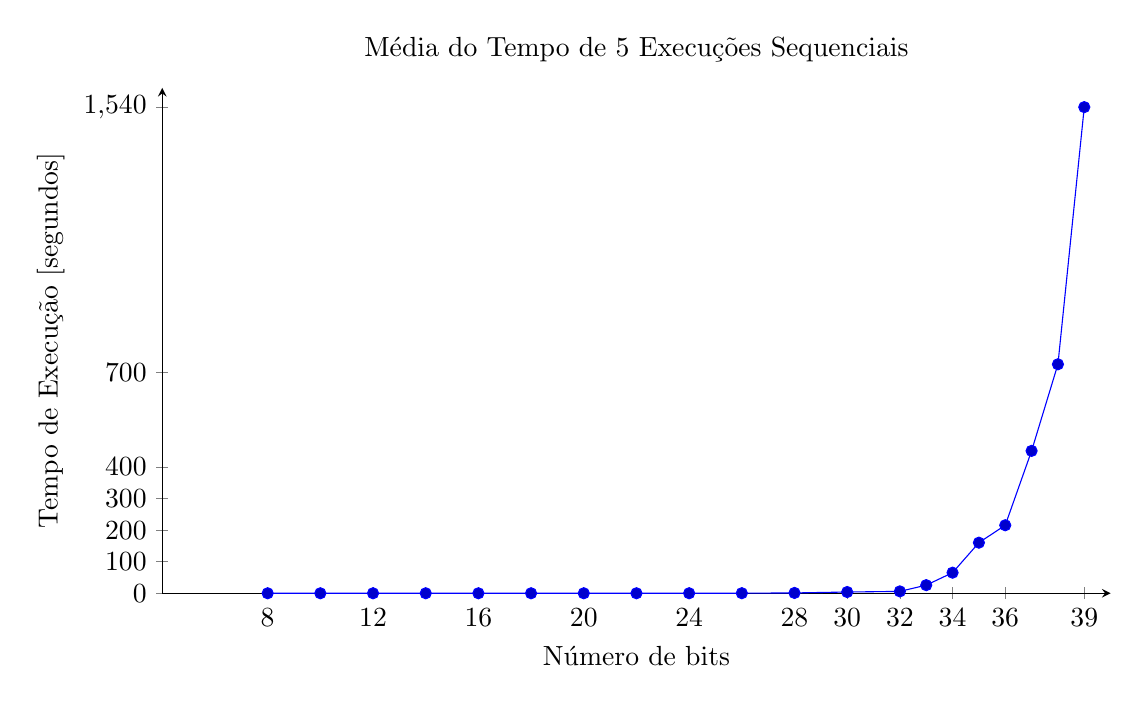
\begin{tikzpicture}
                \begin{axis}[
                    title={Média do Tempo de 5 Execuções Sequenciais},
                    axis lines = left,
                    xlabel={Número de bits},
                    ylabel={Tempo de Execução [segundos]},
                    xmin=4, xmax=40,
                    ymin=0, ymax=1600,
                    xtick={8,12,16,20,24,28,30,32,34,36,39},
                    ytick={0,100,200,300,400,700,1540},
                    legend pos=north east,
                ]
                
                \addplot
                    coordinates {
                        (8, 9.8e-06)(10, 9.4e-06)(12, 1.56e-05)(14, 6.0599999999999996e-05)(16, 0.0001644)(18, 0.000939)(20, 0.0042086)(22, 0.0121472)(24, 0.062906)(26, 0.22889560000000003)(28, 1.04016)(30, 3.92499)(32, 5.983207999999999)(33, 25.687673999999998)(34, 65.173974)(35, 160.16152)(36, 215.34160000000003)(37, 450.76390000000004)(38, 724.9684)(39, 1539.0122)
                    };                    
                \end{axis}
            \end{tikzpicture} 
        \end{adjustwidth}
    \end{frame}

    \begin{frame}{Tempo de Execução Sequenciais}
        \begin{adjustwidth}{-.5cm}{}
            \begin{table}[htbp]
                \begin{tabular}{|c|c|c|c|c|c|}
                    \hline Bits & Tempos (s) & Desvio Padrão & Bits  & Tempo (s)  & Desvio Padrão \\
                    \hline 8    & 9.8e-06    & 0.000001      &  28   & 1.040      & 0.811         \\
                    \hline 10   & 9.4e-06    & 0.000003      &  30   & 3.924      & 1.681         \\
                    \hline 12   & 1.56e-05   & 0.000005      &  32   & 5.983      & 3.844         \\
                    \hline 14   & 6.05e-05   & 0.000065      &  33   & 25.687     & 19.796        \\
                    \hline 16   & 0.0001     & 0.000222      &  34   & 65.173     & 52.038        \\
                    \hline 18   & 0.0009     & 0.000484      &  35   & 160.161    & 61.661        \\
                    \hline 20   & 0.004      & 0.002550      &  36   & 215.341    & 121.509       \\
                    \hline 22   & 0.012      & 0.017561      &  37   & 450.763    & 297.031       \\
                    \hline 24   & 0.0629     & 0.052313      &  38   & 724.968    & 604.576       \\
                    \hline 26   & 0.228      & 0.187669      &  39   & 1539.012   & 1259.526      \\
                    \hline
                \end{tabular}
                \caption{Tempos de Execução Sequencial}
            \end{table}
        \end{adjustwidth}
    \end{frame}

    \begin{frame}{Tempos de Execução Paralelos}
        \begin{adjustwidth}{-1cm}{}
            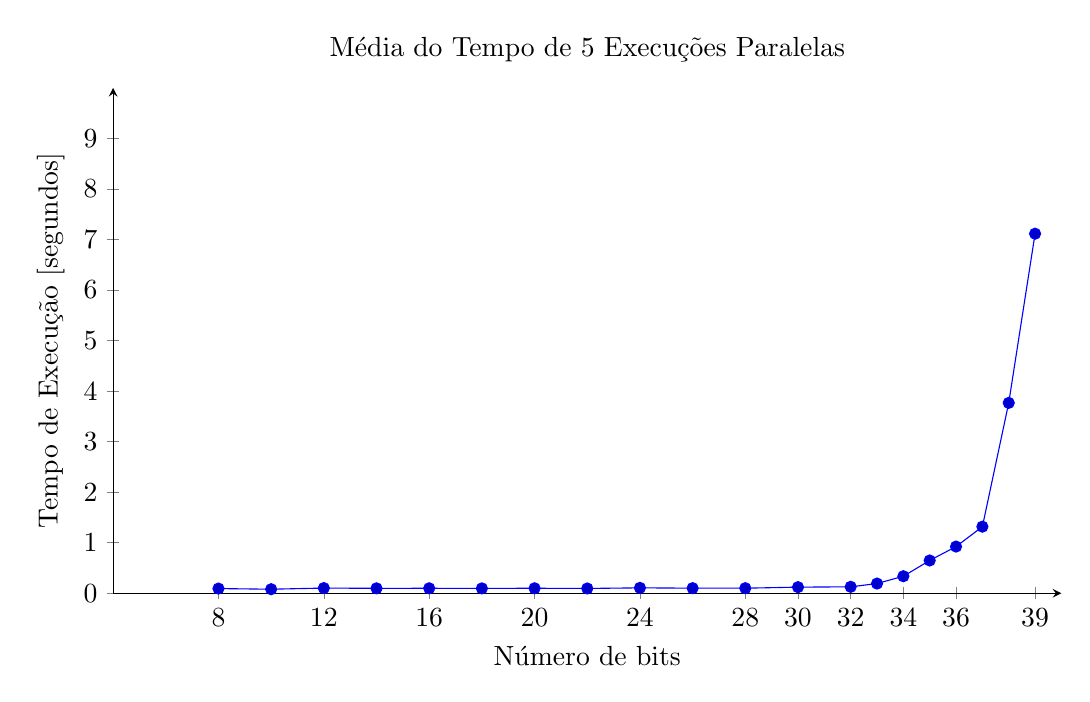
\begin{tikzpicture}
                \begin{axis}[
                    title={Média do Tempo de 5 Execuções Paralelas},
                    axis lines = left,
                    xlabel={Número de bits},
                    ylabel={Tempo de Execução [segundos]},
                    xmin=4, xmax=40,
                    ymin=0, ymax=10,
                    xtick={8,12,16,20,24,28,30,32,34,36,39},
                    ytick={0,1,2,3,4,5,6,7,8,9},
                    legend pos=north east,
                ]
                
                \addplot
                    coordinates {
                        (8,0.0929748)(10,0.080127)(12,0.1028246)(14,0.0976128)(16,0.09850060000000001)(18,0.0966198)(20,0.0990378)(22,0.09520819999999999)(24,0.10716319999999999)(26,0.1010596)(28,0.1004034)(30,0.1210736)(32,0.1275944)(33,0.1921176)(34,0.3372178)(35,0.648707)(36,0.9239993999999999)(37,1.3177906)(38,3.767034)(39,7.114547999999999)
                    };                    
                \end{axis}
            \end{tikzpicture} 
        \end{adjustwidth}
    \end{frame}

    \begin{frame}{Tempo de Execução Paralelo}
        \begin{adjustwidth}{-.5cm}{}
            \begin{table}[htbp]
                \begin{tabular}{|c|c|c|c|c|c|}
                    \hline Bits & Tempos (s) & Desvio Padrão & Bits & Tempo (s) & Desvio Padrão \\
                    \hline 8    & 0.092975   & 0.010403      &  28  & 0.100403  & 0.019439      \\
                    \hline 10   & 0.080127   & 0.012217      &  30  & 0.121074  & 0.016820      \\
                    \hline 12   & 0.102825   & 0.014666      &  32  & 0.127594  & 0.037898      \\
                    \hline 14   & 0.097613   & 0.011124      &  33  & 0.192118  & 0.060779      \\
                    \hline 16   & 0.098501   & 0.009293      &  34  & 0.337218  & 0.124848      \\
                    \hline 18   & 0.096620   & 0.012456      &  35  & 0.648707  & 0.214186      \\
                    \hline 20   & 0.099038   & 0.021616      &  36  & 0.923999  & 0.217719      \\
                    \hline 22   & 0.095208   & 0.013887      &  37  & 1.317791  & 0.606575      \\
                    \hline 24   & 0.107163   & 0.033128      &  38  & 3.767034  & 1.718947      \\
                    \hline 26   & 0.101060   & 0.018860      &  39  & 7.114548  & 4.065866      \\
                    \hline
                \end{tabular}
                \caption{Tempos de Execução Paralelo}
            \end{table}
        \end{adjustwidth}
    \end{frame}

    \begin{frame}{Tempos Sequencial e Paralelo}
        \begin{adjustwidth}{-1cm}{}
            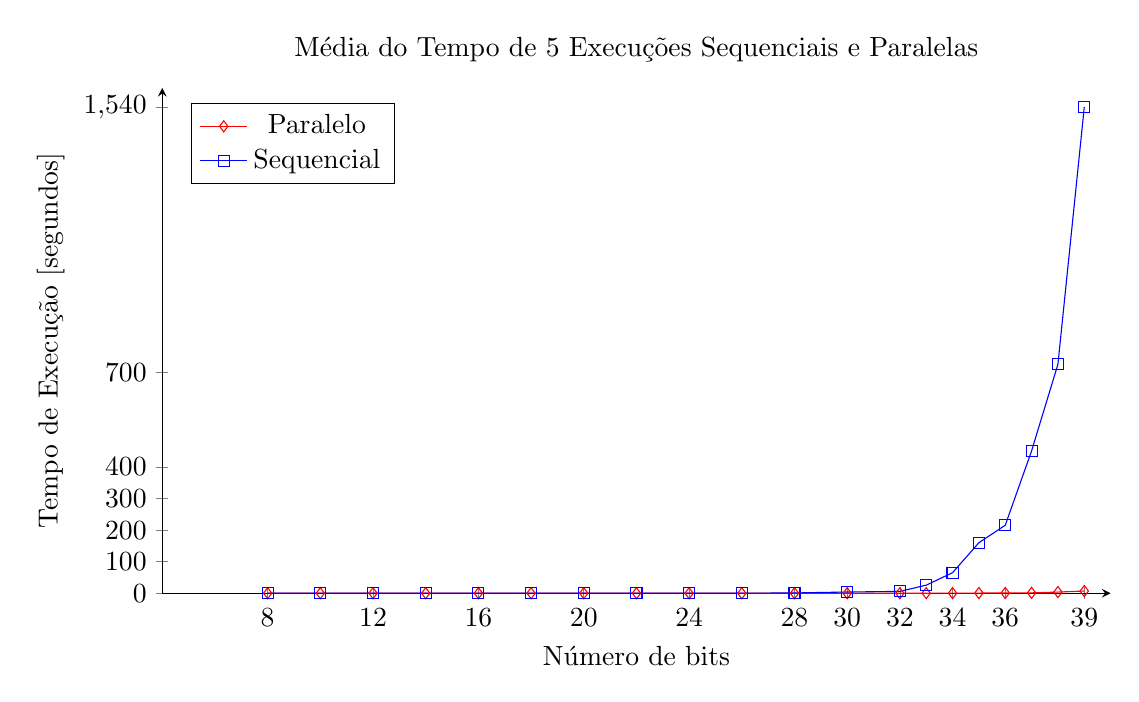
\begin{tikzpicture}
                \begin{axis}[
                    title={Média do Tempo de 5 Execuções Sequenciais e Paralelas},
                    axis lines = left,
                    xlabel={Número de bits},
                    ylabel={Tempo de Execução [segundos]},
                    xmin=4, xmax=40,
                    ymin=0, ymax=1600,
                    xtick={8,12,16,20,24,28,30,32,34,36,39},
                    ytick={0,100,200,300,400,700,1540},
                    legend pos=north west,
                ]
                
                \addplot[
                    color=red,
                    mark=diamond,
                    ]
                    coordinates {
                        (8,0.0929748)(10,0.080127)(12,0.1028246)(14,0.0976128)(16,0.09850060000000001)(18,0.0966198)(20,0.0990378)(22,0.09520819999999999)(24,0.10716319999999999)(26,0.1010596)(28,0.1004034)(30,0.1210736)(32,0.1275944)(33,0.1921176)(34,0.3372178)(35,0.648707)(36,0.9239993999999999)(37,1.3177906)(38,3.767034)(39,7.114547999999999)
                    };
                \addplot[
                        color=blue,
                        mark=square,
                        ]
                        coordinates {
                            (8, 9.8e-06)(10, 9.4e-06)(12, 1.56e-05)(14, 6.0599999999999996e-05)(16, 0.0001644)(18, 0.000939)(20, 0.0042086)(22, 0.0121472)(24, 0.062906)(26, 0.22889560000000003)(28, 1.04016)(30, 3.92499)(32, 5.983207999999999)(33, 25.687673999999998)(34, 65.173974)(35, 160.16152)(36, 215.34160000000003)(37, 450.76390000000004)(38, 724.9684)(39, 1539.0122)
                        };
                \legend{Paralelo,Sequencial}              
                \end{axis}
            \end{tikzpicture} 
        \end{adjustwidth}
    \end{frame}

    \begin{frame}{Speed Up}
        \begin{adjustwidth}{-1cm}{}
            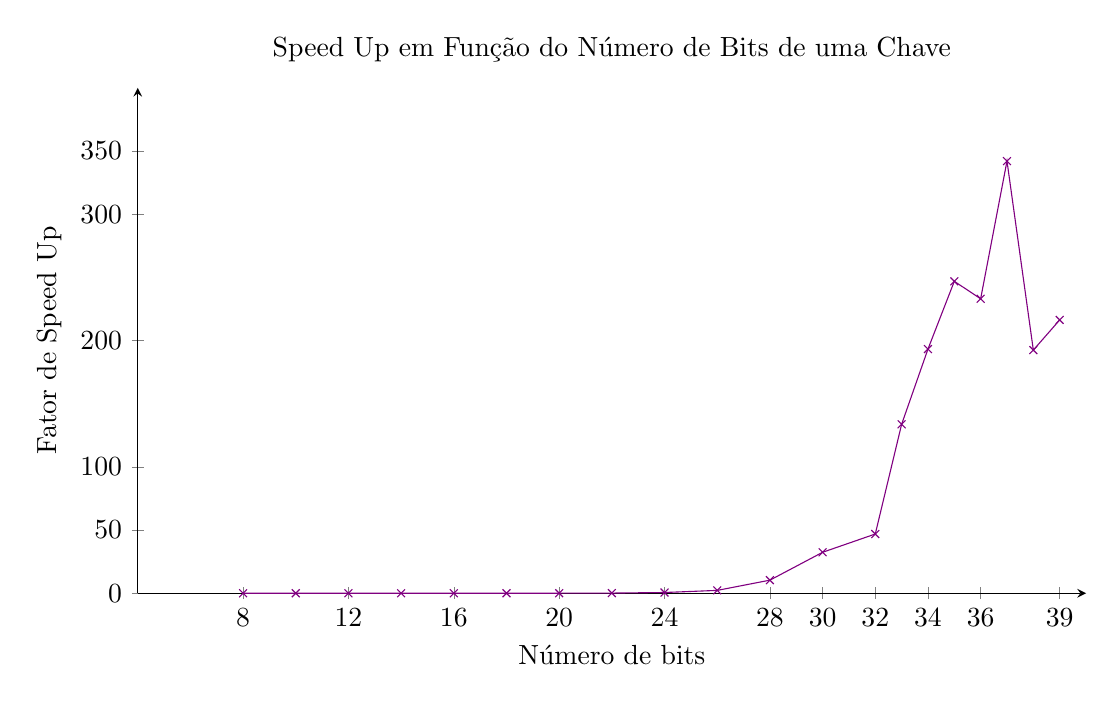
\begin{tikzpicture}
                \begin{axis}[
                    title={Speed Up em Função do Número de Bits de uma Chave},
                    axis lines = left,
                    xlabel={Número de bits},
                    ylabel={Fator de Speed Up},
                    xmin=4, xmax=40,
                    ymin=0, ymax=400,
                    xtick={8,12,16,20,24,28,30,32,34,36,39},
                    ytick={0,50,100,200,300,350},
                    legend pos=north west,
                ]
                
                \addplot[
                    color=violet,
                    mark=x,
                    ]
                    coordinates {
                        (8, 0.0001054049054152308)(10, 0.00011731376439901656)(12, 0.0001517146675017457)(14, 0.0006208202202989771)(16, 0.0016690253663429462)(18, 0.009718504902721801)(20, 0.042494885791081786)(22, 0.12758564913526357)(24, 0.5870112128043956)(26, 2.264956520706593)(28, 10.359808532380377)(30, 32.41821503614331)(32, 46.89240280137686)(33, 133.7080725555597)(34, 193.2696731904425)(35, 246.89346654190564)(36, 233.0538309873362)(37, 342.06033948033934)(38, 192.45071852284846)(39, 216.31904092853125)
                    };
                \end{axis}
            \end{tikzpicture} 
        \end{adjustwidth}
    \end{frame}

    \begin{frame}{Speed Up e Eficiência}
        \begin{adjustwidth}{-.5cm}{}
            \begin{table}[htbp]
                \begin{tabular}{|c|c|c|c|c|c|}
                    \hline Bits & SpeedUp & Eficiência & Bits & SpeedUp & Eficiência \\
                    \hline 8    & 0.00    & 0.00 \%    &  28  & 10.36   & 16.19  \%  \\
                    \hline 10   & 0.00    & 0.00 \%    &  30  & 32.42   & 50.65  \%  \\
                    \hline 12   & 0.00    & 0.00 \%    &  32  & 46.89   & 73.27  \%  \\
                    \hline 14   & 0.00    & 0.00 \%    &  33  & 133.71  & 208.92 \%  \\
                    \hline 16   & 0.00    & 0.00 \%    &  34  & 193.27  & 301.98 \%  \\
                    \hline 18   & 0.01    & 0.02 \%    &  35  & 246.89  & 385.77 \%  \\
                    \hline 20   & 0.04    & 0.07 \%    &  36  & 233.05  & 364.15 \%  \\
                    \hline 22   & 0.13    & 0.20 \%    &  37  & 342.06  & 534.47 \%  \\
                    \hline 24   & 0.59    & 0.92 \%    &  38  & 192.45  & 300.70 \%  \\
                    \hline 26   & 2.26    & 3.54 \%    &  39  & 216.32  & 338.00 \%  \\
                    \hline
                \end{tabular}
                \caption{Speed Up e Eficiência}
            \end{table}
        \end{adjustwidth}
    \end{frame}

    \begin{frame}{Testes Extras}
        \begin{adjustwidth}{-1cm}{}
            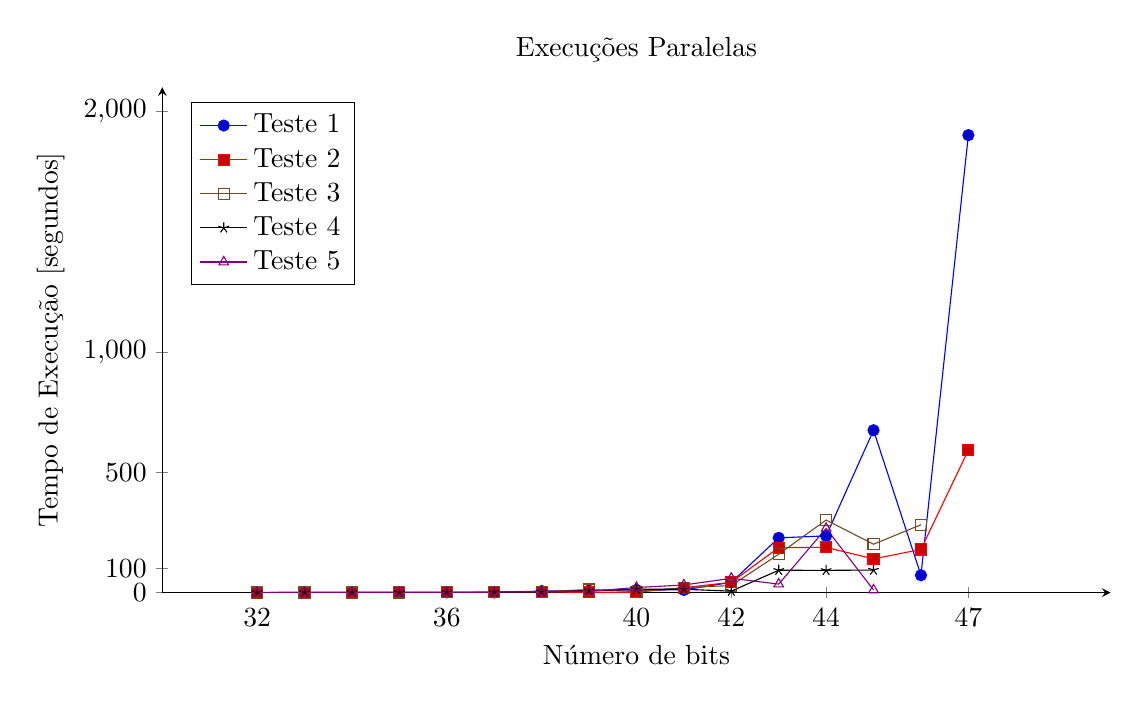
\begin{tikzpicture}
                \begin{axis}[
                    title={Execuções Paralelas},
                    axis lines = left,
                    xlabel={Número de bits},
                    ylabel={Tempo de Execução [segundos]},
                    xmin=30, xmax=50,
                    ymin=0, ymax=2100,
                    xtick={32,36,40,42,44,47},
                    ytick={0,100,500,1000,2000},
                    legend pos=north west,
                ]
                
                \addplot
                    coordinates {
                        (32, 0.181284)(33, 0.204819)(34, 0.371035)(35, 0.309007)(36, 1.03462)(37, 0.572565)(38, 6.33488)(39, 8.19878)(40, 10.8017)(41, 11.1191)(42, 42.7333)(43, 227.549)(44, 235.577)(45, 674.659)(46, 72.0661)(47, 1900.89)
                    };
                \addplot
                    coordinates {
                        (32, 0.111628)(33, 0.15273)(34, 0.335075)(35, 0.881869)(36, 0.85777)(37, 1.26508)(38, 1.7281)(39, 1.58637)(40, 1.56563)(41, 20.2721)(42, 42.8525)(43, 186.925)(44, 188.031)(45, 139.913)(46, 179.342)(47, 592.411)
                    };
                \addplot+[mark=square]
                    coordinates {
                        (32, 0.104469)(33, 0.112361)(34, 0.151638)(35, 0.754069)(36, 1.17011)(37, 2.1112)(38, 3.55764)(39, 12.6372)(40, 4.17425)(41, 20.5217)(42, 29.3224)(43, 159.559)(44, 301.434)(45, 201.039)(46, 281.908)
                    };
                \addplot
                    coordinates {
                        (32, 0.088942)(33, 0.268117)(34, 0.327808)(35, 0.612964)(36, 0.966121)(37, 0.943168)(38, 2.90973)(39, 7.86113)(40, 14.1505)(41, 13.8583)(42, 6.04276)(43, 92.8612)(44, 92.3861)(45, 93.6913)
                    };
                \addplot[color=violet,mark=triangle]
                    coordinates {
                        (32, 0.151649)(33, 0.222561)(34, 0.500533)(35, 0.685626)(36, 0.591376)(37, 1.69694)(38, 4.30482)(39, 5.28926)(40, 21.1594)(41, 31.6205)(42, 59.2854)(43, 35.2571)(44, 266.691)(45, 11.0068)
                    };
                \legend{Teste 1, Teste 2, Teste 3, Teste 4, Teste 5}
                \end{axis}
            \end{tikzpicture} 
        \end{adjustwidth}
    \end{frame}
\end{document}
